\documentclass[12pt]{article}
\usepackage{geometry}
\geometry{
	a4paper,
	margin=2cm,
	left=3cm, bottom=2.5cm}

\usepackage[utf8]{inputenc}
\usepackage[german]{babel}
\usepackage[T1]{fontenc}
\usepackage{hyperref}
\usepackage{listings}
\usepackage{graphicx}
\usepackage{color}
\usepackage[toc]{glossaries}
\usepackage{chngcntr} %change counter
\usepackage{tabularx}
\usepackage{fancyhdr}
\usepackage{rotating} 
\usepackage{lscape}	% querformat
%predefined colors: black, blue, cyan, green, magenta, red, white, yellow
\definecolor{commentgreen}{rgb}{0,0.6,0}
\definecolor{keywordblue}{rgb}{0,0,0.8}
\definecolor{orange}{rgb}{0.9,0.5,0}
\definecolor{internal_link}{rgb}{0,0,0.4}

\hypersetup{
	colorlinks=true, 
	linkcolor=internal_link, 
	urlcolor=cyan}

\lstset{
	language=C,
	basicstyle=\footnotesize\ttfamily,
	showstringspaces=false,
	commentstyle=\itshape\color{commentgreen},
	keywordstyle=\bfseries\color{keywordblue},
%	identifierstyle=\color{red},
	stringstyle=\color{orange}
}

\setlength{\parindent}{0em} %setzt Paragraphen-Einzug auf 0
\renewcommand{\labelitemi}{\textbullet}
\renewcommand\labelitemii{\textbullet}
\renewcommand\labelitemiii{\textbullet}
\renewcommand{\theenumi}{\arabic{enumi}}
\renewcommand{\theenumii}{\arabic{enumii}}
\renewcommand{\theenumiii}{\arabic{enumiii}}

\makeglossaries
%bash: (glossaries = filename)
%pdflatex glossaries.tex
%makeglossaries glossaries
%pdflatex glossaries.tex 

\title{\textbf{Pflichtenheft}}
\author{"Interaktives \Gls{TicTacToe} für Kinder"}
\date{\today} %richtige Formatierung mittels package babel (s.o.)


\newglossaryentry{TicTacToe}{
	name= TicTacToe,
	description = {Strategiespiel dessen Wurzeln im 12. Jahrhundert vor Christus liegen}
}

\newglossaryentry{Empfangstresen}{
	name= Empfangstresen,
	description = {Bereich zur Aufnahme der erschienen Patienten}
}

\newglossaryentry{Sprechstunde}{
	name= Sprechstunde,
	description = {Öffnungszeit der Kinderarztpraxis, in der die Behandlung von Patienten erfolgt}
}

\newglossaryentry{Icon}{
	name= Icon,
	description = {Kleines Bildsymbol}
}
\newglossaryentry{Button}{
	name= Button,
	description = {Betätigbare Schaltfläche },
	plural=Buttons
}
\newglossaryentry{CLI}{
	name= CLI,
	description = {Entspricht "Command Line Interface"}
}
\newglossaryentry{Repository}{
	name= Repository,
	description = {Ein Raum, Container wo etwas zur Aufbewahrung gespeichert werden soll}
}


\pagestyle{fancy}
\renewcommand{\headrulewidth}{0pt}
\fancyhf{}
\cfoot{
\includegraphics[scale=0.9]{footer.pdf} \thepage}

\begin{document}
\begin{titlepage}
	\centering	
	\begin{figure}
	
\includegraphics[scale=0.9]{banner.pdf} %\logo{
\includegraphics{banner.pdf}}
	\end{figure}
	\maketitle
	\thispagestyle{empty}
	
	\vspace*{1cm}	
	
	\begin{flushleft}
	Stand:\hspace*{31mm}30.01.2019\\
	Auftraggeber:\hspace*{17mm}Kinderarztpraxis Dr. med. Lasse Niessen\\
	Kontakt:\\
		\hspace*{5mm}Ansprechpartner:\hspace*{6mm}Dr. med. Lasse Niessen\\
		\hspace*{5mm}Telefon:\hspace*{23mm}0351/327890\\
		\hspace*{5mm}Adresse:\hspace*{22mm}Kinderarztpraxis Dr. med. Lasse Niessen\\
							\hspace*{42mm}Spielerstr. 56\\
							\hspace*{42mm}D-01069 Dresden\\
	
	Öffnungszeiten:\\
		\hspace*{42mm}Montag bis Samstag\\
		\hspace*{42mm}7:00 Uhr - 17:00 Uhr\\
	\end{flushleft}

	\vspace*{1cm}
	
	\begin{flushleft}
	Auftragnehmer:\hspace*{14mm}Kleinprogramm GmbH \\
	Kontakt:\\
		\hspace*{5mm}Ansprechpartner:\hspace*{6mm}Michael Leopold\\
		\hspace*{5mm}Telefon:\hspace*{23mm}0351/654321\\
		\hspace*{5mm}Adresse:\hspace*{22mm}Kleinprogramm GmbH\\
		\hspace*{42mm}Eichenweg 6\\
		\hspace*{42mm}D-01069 Dresden\\	
		\hspace*{42mm}kontakt@kp.de
	\end{flushleft}
	\newpage \thispagestyle{empty} \tableofcontents 
\end{titlepage}

%"` links, "' rechts

\setcounter{page}{3}

\section{Zielbestimmung}
Für die Kinderartzpraxis von Dr. med. Lasse Niessen soll eine interaktive, per Touchscreen bedienbare, "`\Gls{TicTacToe}"' Anwendung in Java entwickelt werden. Dies soll dazu dienen Kindern den Umgang mit Technik im Alltag spielerisch beizubringen.

Es soll ein Programm entstehen, dass beim Aufruf direkt im Vollbild-Modus startet. Es soll nicht möglich sein, dass die Anwender des Spiels die Anwendung schließen können. Dies soll nur über die Rezeption der Arztpraxis geschehen.

\subsection{Muss-Kriterien}
\begin{tabularx}{\textwidth}{|l|l|X|} \hline
MK-IO-01&Output&Das System muss im Vollbild-Modus starten.\\ \hline
MK-IO-02&Output&Das System muss nach dem Start zuerst ein Menü anzeigen, in dem als Titel der Name des Spiels und als anwählbare \Glspl{Button} "`Spiel starten"', "`Regeln"' und "`Infos"' existieren.\\ \hline
MK-IO-03&Input &Die Eingabe muss durch die Berührung des Bildschirms erfolgen.\\ \hline
MK-SYS-01&OO-Analyse&Die Analyse des Systems muss objektorientiert erfolgen.\\ \hline
MK-SYS-01&UML2&Für die Modellierung und Dokumentation muss UML2 genutzt werden.\\ \hline
MK-IMPL-01&JavaCode&Implementierung muss in Java erfolgen.\\ \hline
MK-IMPL-02&CodeStyle&Der Quellcode ist nach den Vorgaben des Google Java Style Guide zu implementieren\\&&(https://google.github.io/styleguide/javaguide.html).\\ \hline
\end{tabularx}\\

\subsection{Kann-Kriterien}
\begin{tabularx}{\textwidth}{|l|l|X|} \hline
KK-BS-01&Anzeige, Hilfe&Das System kann auf der vorgesehenen Ausgabe Informationen zur Firma, Praxis, Programmierer anzeigen.\\ \hline
\end{tabularx}\\

\subsection{Abgrenzungskriterien}
\begin{tabularx}{\textwidth}{|l|l|X|} \hline
AK-IO-01&GUI&Das System soll kein \Gls{CLI} haben.\\ \hline
AK-T-01&Testung&Das System soll keinen Usability-Test durchlaufen.\\ \hline
\end{tabularx}\\

%%%%
\section{Produkteinsatz}
\subsection{Anwendungsbereich}
Die \Gls{TicTacToe}-Anwendung dient dem förderlichem Umgang mit Technik bei Kindern. Eltern und Kinder können die Wartezeit in der Praxis angenehmer gestalten. Die soziale Interaktion der Patienten wird außerdem gefördert.
\subsection{Zielgruppen}
Benutzt wird die Anwendung von Patienten bzw. Besuchern und Angestellten der Kinderarztpraxis Dr. med. Lasse Niessen. Dabei werden Kinder und Eltern die Hauptrolle einnehmen. Die Angestellten der Kinderarztpraxis sind für das Starten und Beenden der Anwendung zuständig. Weitere Rollen - wie beispielsweise eine Administratorrolle - treten nicht auf.
\subsection{Produktumgebung}
Das System benötigt mindestens eine installierte Java Runtime ab Java-Version 1.8. Um mit wenig Aufwand starten zu können, ist der Bin-Ordner der Javaumgebung in der globalen Pfad-Variable des Betriebssystems abzulegen.
Hardwarederungen bestehen in dem Touchscreen, welcher mit einem Bildschirm verbunden sein muss. Dieser ist bereits vorhanden.
\subsubsection{Architektur}
Die verwendete Architektur ist ein 64bit-Windows-10-Betriebssystem.
\subsection{Betriebsbedingungen}
Das System wird für die Anwendungsfälle F1 und F2 im Warteraum beziehungsweise am Empfang der Kinderarztpraxis genutzt. Die Angestellten öffnen die Anwendung an dem dort befindlichen Rechner, während die Hauptnutzer im Wartezimmer spielen. Die Anwendung soll ohne weitere Betreuung durch das Praxispersonal funktionieren, um den Praxisalltag nicht zu beeinflussen. Der Rechner wird zyklisch aktualisiert und es läuft ein Windows 10 Betriebssystem ab der Version 1809. Die Wartung beziehungsweise Installation der Software erfolgt außerhalb der Sprechzeiten oder in Pausenzeiten der Praxis, die mindestens 30 Minuten betragen. Der Raum ist klimatisiert. Der Rechner hat keine unterbrechungsfreie Stromversorgung.

%%%%
\section{Produktfunktionen/Anforderung}
\subsection{Funktionale Anforderungen}
\subsubsection{Beschreibung der Funktionalen Anforderungen mit Rollen innerhalb der Geschäftsprozesse}
\begin{tabularx}{\textwidth}{|l|l|X|} \hline
AF-01&Programmstart&Das Programm soll in ein Menü mit dem Titel "`\Gls{TicTacToe}"' starten, in dem weiterhin die \Glspl{Button} "`Spiel starten"', "`Regeln"', "`Infos"'.\\ \hline
AF-02&Spielen&Das Spiel soll über die Berührung des "`Spiel starten"'-\Glspl{Button} gestartet werden. Es soll die Spielfläche von 3x3 Feldern angezeigt werden. Durch die Berührung von jeweils einem noch freien Spielfeld soll auf dem gewählten Spielfeld das Symbol des jeweiligen Spieler erscheinen.\\ \hline
AF-03&Gewinnauswertung&Das Programm analysiert nach jedem Spielzug das Spiel und erkennt, wenn ein Spieler gewonnen hat oder ein Unentschieden entsteht. Tritt einer dieser Fälle ein, wird das Spielfeld ausgeblendet und eine Meldung gezeigt, die das Spielergebnis beschreibt. Weiterhin soll es zwei \Glspl{Button} geben: "`Neues Spiel starten"', welcher ein neues Spiel beginnt, und "`zurück zum Menü"', welcher bei Aktivierung wieder das Menü anzeigt.\\ \hline
AF-04&Testung 1&Es wird zunächst ein einfacher Funktionstest für den Anwendungsfall AF-05 gemacht. \\ \hline
AF-05&Testung 2&Im Einsatz soll in der ersten Woche die Wirkung auf die Kinder durch das Personal überprüft werden. Bei Fehlfunktion beziehungsweise schlechter Annahme wird eine Überarbeitung angestrebt.\\ \hline
AF-06&Starten&ausschließlich durch Mitarbeiter, per Touch-Eingabe über eine Desktop-Verknüpfung\\ \hline
AF-07&Beenden&ausschließlich durch Mitarbeiter, durch Rechtsklick auf das Symbol in der Taskleiste -> Fenster schließen\\ \hline
AF-08&Auflösung&Die Auflösung wird im 16:9 Format und mit 1920x1080 Pixeln realisiert und dafür optimiert.\\ \hline
\end{tabularx}\\\\

\subsubsection{Aktivitäten mit Benutzerschnittstelle (UI)}
\begin{tabularx}{\textwidth}{|l|X|} \hline
Anwendungsfall ID&AF-01\\ \hline
AF Name&Programm starten\\ \hline
Akteur&Mitarbeiter\\ \hline
Vorbedingung&Pfad-Variable auf den bin-Ordner der Javaumgebung ist gesetzt\\ \hline
Auslösendes Ereignis&Programmstart\\ \hline
Nachbedingung Erfolg&Fenster öffnet sich\\ \hline
Nachbedingung Fehlschlag&Programm konnte nicht gestartet werden\\ \hline
Ablauf&- Doppelklick auf ausführbare Datei\\&- Ausgabe des Fensters erfolgt \\ \hline
Benutzerschnittstelle&
\includegraphics[scale=0.33]{Beenden.pdf} \\ \hline
\end{tabularx}\\

\begin{tabularx}{\textwidth}{|l|X|} \hline
Anwendungsfall ID&AF-02\\ \hline
AF Name&Menue anzeigen\\ \hline
Akteur&Patienten als Spieler\\ \hline
Vorbedingung&Fenster ist geöffnet\\ \hline
Auslösendes Ereignis&Programmstart oder Touch-Eingabe auf einen "`zurück zum Menü"'-\Gls{Button}\\ \hline
Nachbedingung Erfolg&Ausgabe des Menüs erfolgt auf Bildschirm\\ \hline
Nachbedingung Fehlschlag& \\ \hline
Ablauf&- Programm wurde gestartet oder Touch-Eingabe auf einen "`zurück zum Menü"'-\Glspl{Button}\\&- Ausgabe Menü erfolgt \\ \hline
Benutzerschnittstelle&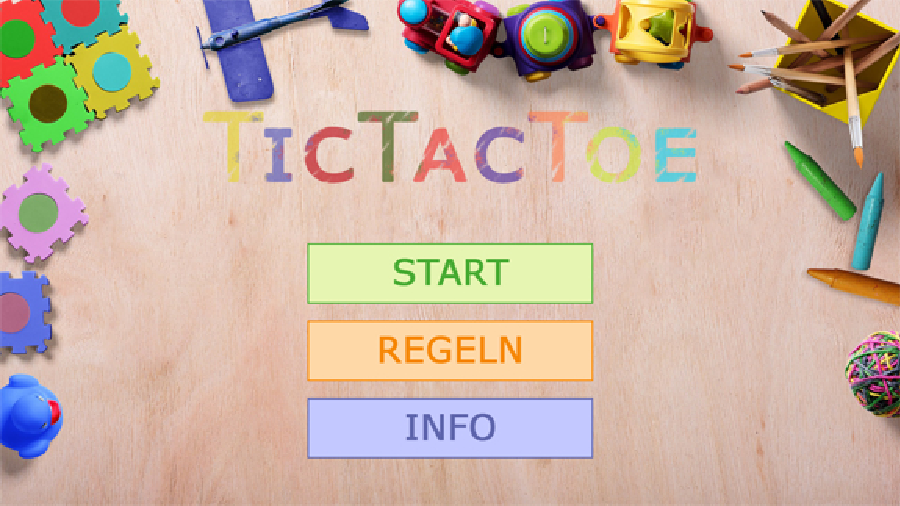
\includegraphics[scale=0.33]{Menu.pdf} \\ \hline
\end{tabularx}\\

\begin{tabularx}{\textwidth}{|l|X|} \hline
Anwendungsfall ID&AF-03\\ \hline
AF Name&Regeln anzeigen\\ \hline
Akteur&Patienten als Spieler\\ \hline
Vorbedingung&Menü wird angezeigt\\ \hline
Auslösendes Ereignis&Touch-Eingabe auf den "`Regeln"'-\Gls{Button}\\ \hline
Nachbedingung Erfolg&Ausgabe der Regeln erfolgt auf Bildschirm\\ \hline
Nachbedingung Fehlschlag&Menü wird weiterhin angezeigt\\ \hline
Ablauf&- Eingabe auf den "`Regeln"'-\Gls{Button}\\&- Regeln werden angezeigt\\ \hline
Benutzerschnittstelle&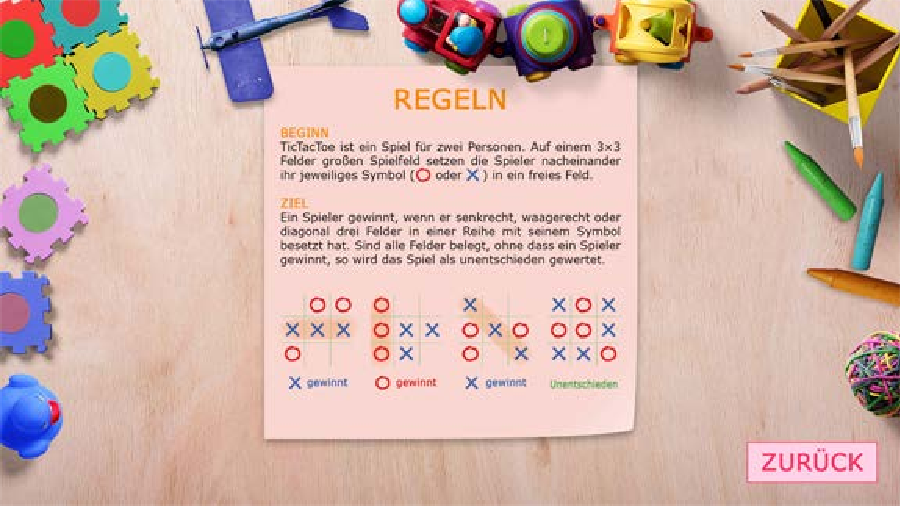
\includegraphics[scale=0.33]{Regeln.pdf}\\ \hline
\end{tabularx}\\

\begin{tabularx}{\textwidth}{|l|X|} \hline
Anwendungsfall ID&AF-04\\ \hline
AF Name&Infos anzeigen\\ \hline
Akteur&Patienten als Spieler\\ \hline
Vorbedingung&Menü wird angezeigt\\ \hline
Auslösendes Ereignis&Touch-Eingabe auf den "`Infos"'-\Gls{Button}\\ \hline
Nachbedingung Erfolg&Ausgabe der Informationen erfolgt auf Bildschirm\\ \hline
Nachbedingung Fehlschlag&Menü wird weiterhin angezeigt\\ \hline
Ablauf&- Eingabe auf den "`Infos"'-\Gls{Button}\\&- Infos werden angezeigt\\ \hline
Benutzerschnittstelle&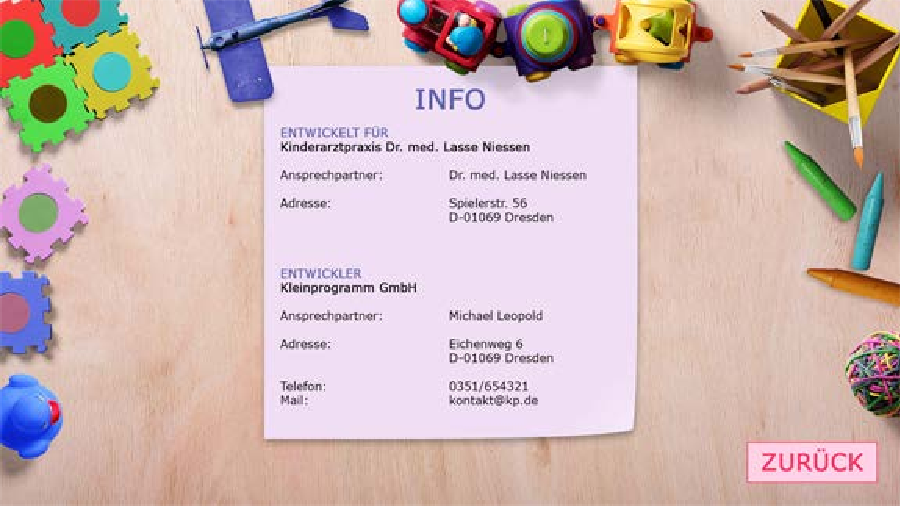
\includegraphics[scale=0.33]{Info.pdf}
\\ \hline
\end{tabularx}\\

\begin{tabularx}{\textwidth}{|l|X|} \hline
Anwendungsfall ID&AF-05\\ \hline
AF Name&Spiel spielen\\ \hline
Akteur&Patienten als Spieler\\ \hline
Vorbedingung&Menü wird angezeigt\\ \hline
Auslösendes Ereignis&Touch-Eingabe auf den "`Spielen"'-\Gls{Button}\\ \hline
Nachbedingung Erfolg&Ausgabe des Spielfelds erfolgt auf Bildschirm\\ \hline
Nachbedingung Fehlschlag&Menü wird weiterhin angezeigt\\ \hline
Ablauf&- Eingabe auf den "`Spielen"'-\Gls{Button}\\&- Spielfeld wird angezeigt\\&- Spieler tätigt Eingabe\\ \hline
Benutzerschnittstelle&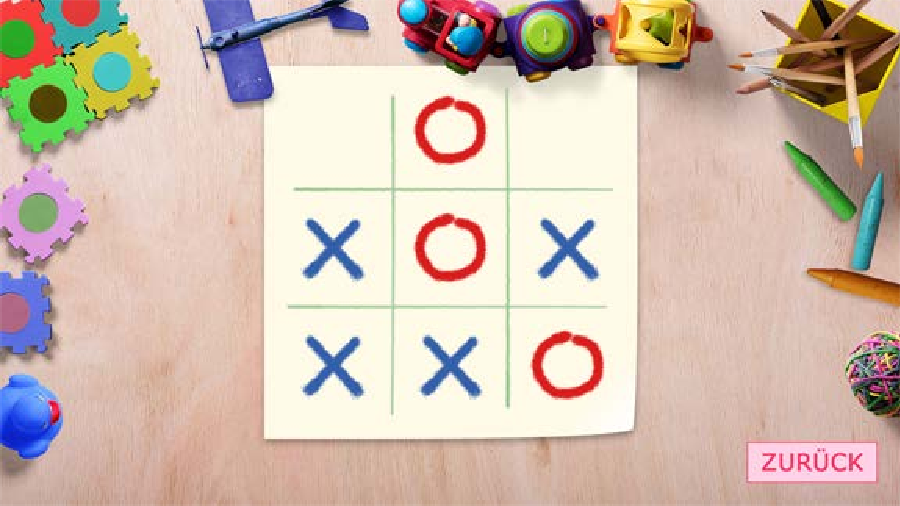
\includegraphics[scale=0.33]{Spielen.pdf}\\ \hline
\end{tabularx}\\

\begin{tabularx}{\textwidth}{|l|X|} \hline
Anwendungsfall ID&AF-06\\ \hline
AF Name&Programm beenden\\ \hline
Akteur&Mitarbeiter\\ \hline
Vorbedingung&Programm ist gestartet\\ \hline
Auslösendes Ereignis&Tasteneingabe <ALT>+<F4> oder Rechtsklick auf \Gls{Icon} in Taskleiste mit gewählter Option "`Fenster schließen"'\\ \hline
Nachbedingung Erfolg&Fenster wird geschlossen\\ \hline
Nachbedingung Fehlschlag&Fenster schließt sich nicht\\ \hline
Ablauf&- Tasteneingabe <ALT>+<F4>\\&- Fenster wird geschlossen\\ \hline
Benutzerschnittstelle&
\includegraphics[scale=0.33]{Beenden.pdf}\\ \hline
\end{tabularx}\\

\newpage
\subsubsection{Fachliches Klassendiagramm (domain model) / Produktdaten}
Für die \Gls{TicTacToe}-Anwendung sind keine Daten dauerhaft zu speichern. \\
%\begin{landscape}
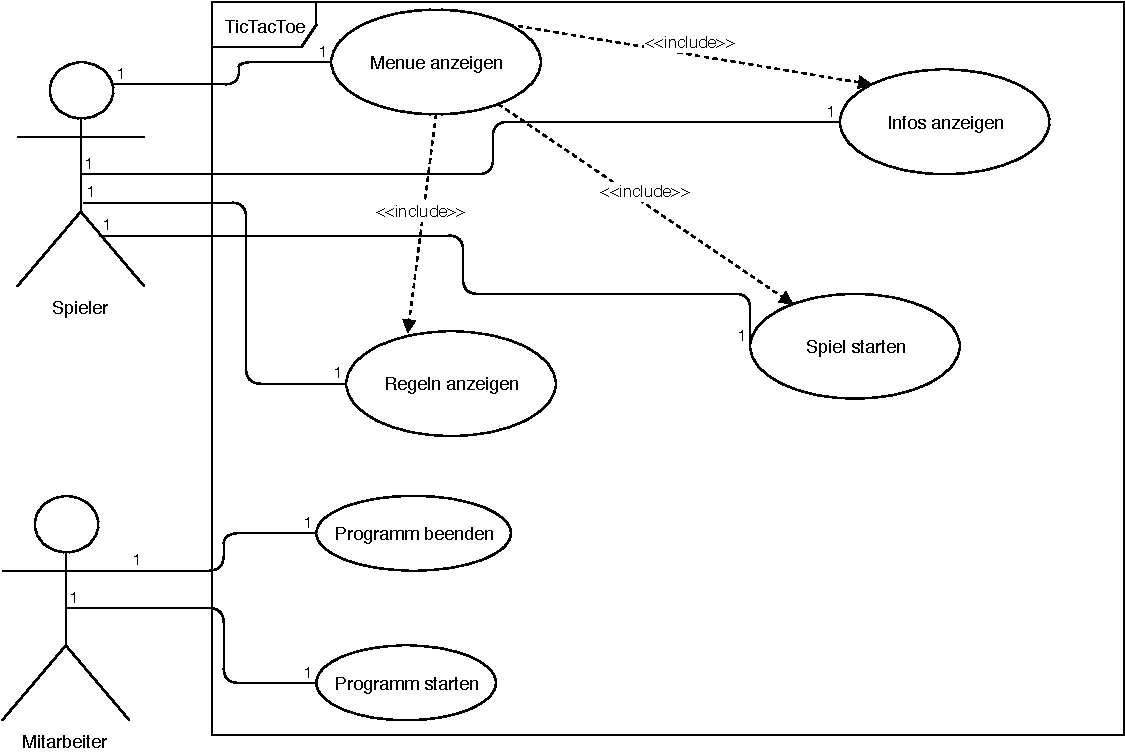
\includegraphics[scale=0.9]{Anwendungsfalldiagramm.pdf}\\

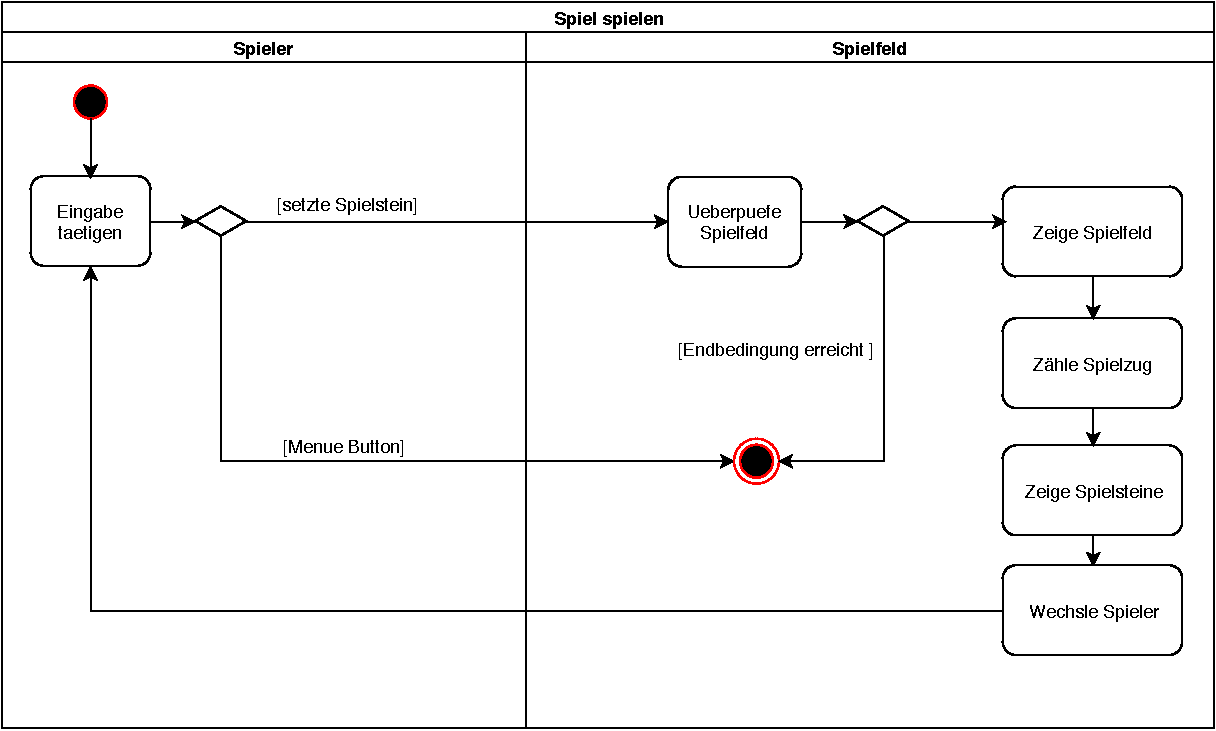
\includegraphics[scale=0.85]{Aktivitaetsdiagramm.pdf}
\vspace{5cm}
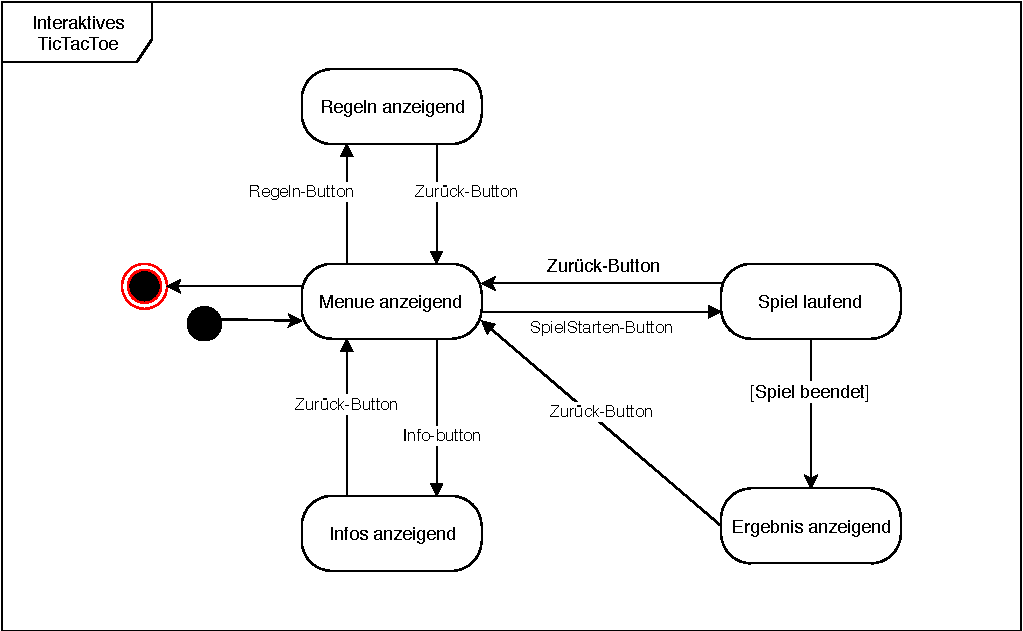
\includegraphics[scale=0.9]{Zustandsdiagramm.pdf}\\

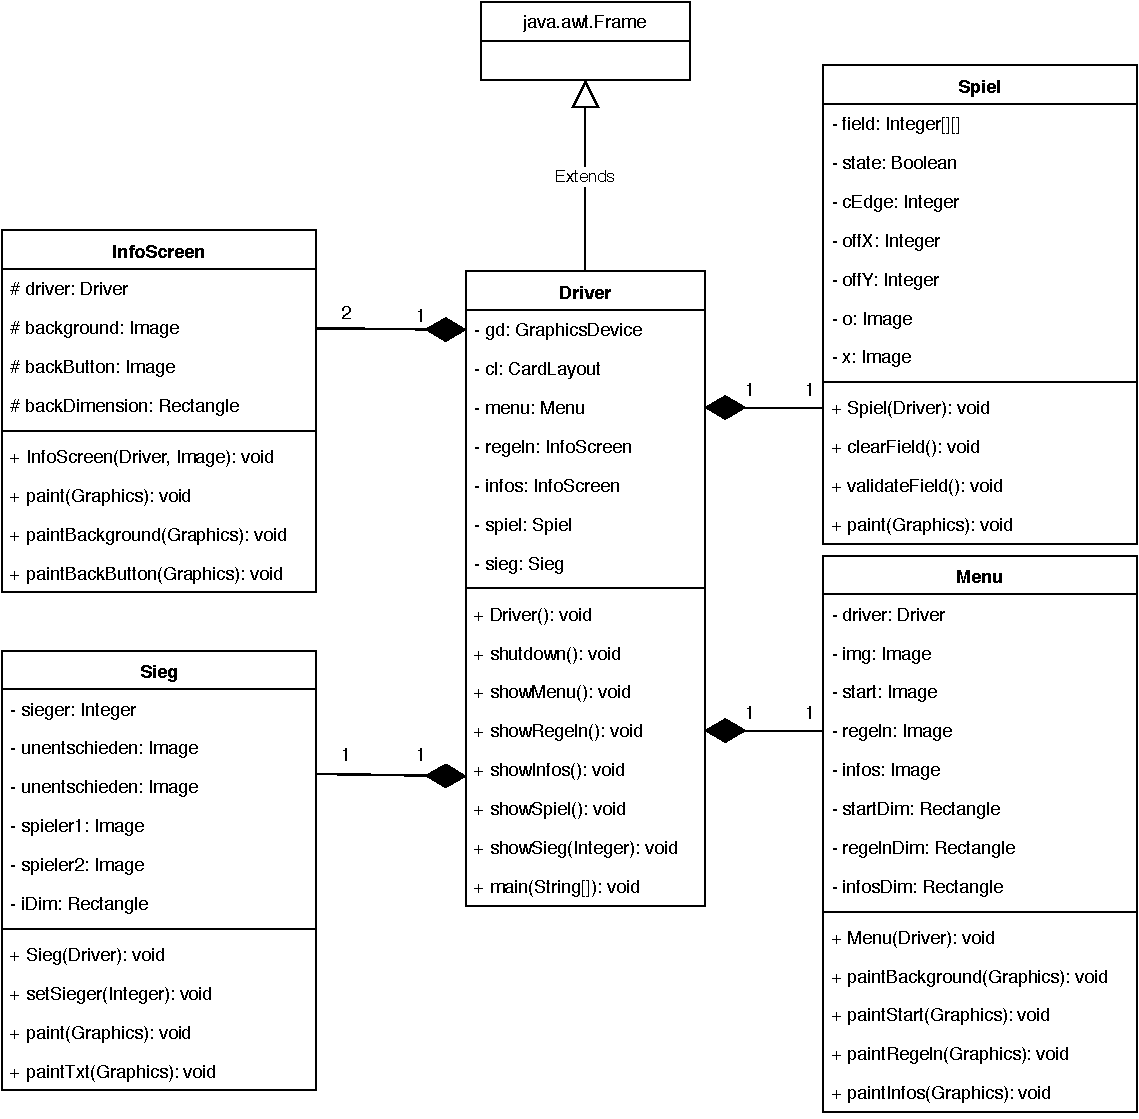
\includegraphics[scale=0.85]{Klassendiagramm.pdf}
%\end{landscape}
\subsection{Nichtfunktionale Anforderungen} 
%Benutzbarkeit, Zuverlässigkeit, Effizienz, Softwarewartung, Sicherheit, Normen
\begin{tabularx}{\textwidth}{|X|X|X|} \hline
NF-B1&Benutzung&\Gls{TicTacToe} soll nur mittels der GUI auf einem separaten Monitor genutzt werden.\\ \hline
NF-E1&Effizienz&Die Nutzereingabe soll unmittelbar angezeigt werden\\ \hline
NF-W1&Softwarewartung&Es ist langfristig vorgesehen noch weitere Spiele und ein Spiele verwaltendes Menü hinzuzufügen. \\ \hline
\end{tabularx}\\
%%%%
\section{Testung}
Funktionstests werden gemäß der Anwendungsfälle AF-04 und AF-05 durchgeführt.

%\tbf{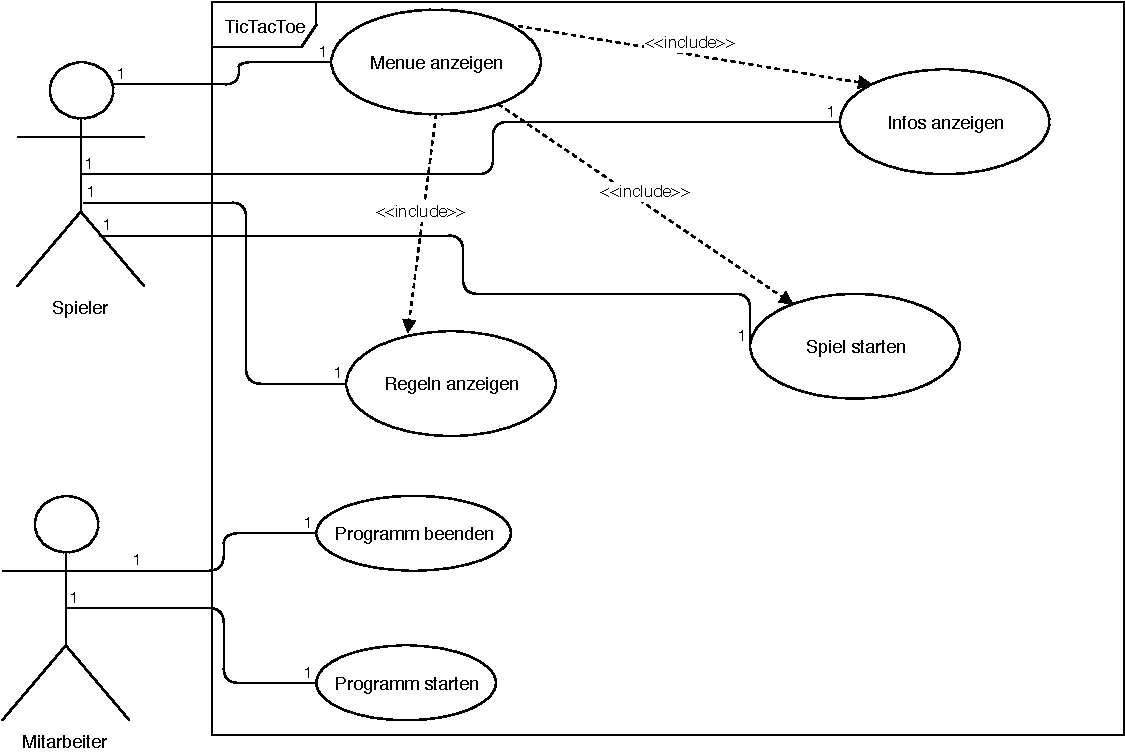
\includegraphics[scale=0.5]{Anwendungsfalldiagramm.pdf}}
%%%%
\section{Monitoring/Support bei der Übergabe oder ähnliche Leistungen}
Die Erstinstallation wird außerhalb der Geschäftszeiten des AG erfolgen. Der Auftraggeber sowie dessen Angestellte werden einmalig in die Funktionsweise des Programms eingewiesen. Ein \Gls{Repository} wird zur Verfügung gestellt. Rufbereitschaft wochentags 8-17 Uhr per E-Mail ist gewährleistet. 

%%%%
\section{Dokumentation}
\subsection{Anwenderdokumentation}
Die Anwenderdokumentation wird als readme.pdf Datei in deutscher Sprache zur Verfügung gestellt.
\subsection{Administratorendokumentation}
Eine Dokumentation für Administratoren ist nicht vorgesehen.
\subsection{Entwicklerdokumentation}
Als Entwicklerdokumentation werden die mit javadoc generierten HTML-Dokumente im \Gls{Repository} zur Verfügung gestellt.
\subsection{Weitere referenzierte Dokumente}
Das Pflichtenheft wurde anhand des Lastenhefts "`Interaktives \Gls{TicTacToe} für Kinder"' erstellt. Lastenheft, Pflichtenheft und die Anwenderdokumentation befinden sich im \Gls{Repository}.
%%%%
\newpage
\section{Vorgehen}
Für den Anwendungsfall AF-01 und AF-02 wird ein Prototyp erstellt, der gemäß der nicht funktionalen Anforderungen inkrementell erweitert wird. Danach erfolgt der Funktionstest. Diese letzte Testversion gilt als Release Candidate auf deren Basis auch die Dokumentation abgeschlossen wird. Anschließend erfolgt die Übergabe.\\
Meilensteine:\\\\
\begin{tabularx}{\textwidth}{|X|X|} \hline
\textbf{Datum}&\textbf{Meilenstein}\\ \hline
18.03.2019&Vorbereitung\\ \hline
29.03.2019&Projektplan und Pflichtenheft\\ \hline
12.04.2019&Analyse und Entwurf\\ \hline
03.05.2019&Prototyp\\ \hline
10.05.2019&Funktionstest gemäß AF-04\\ \hline
30.08.2019&Release\\ \hline
13.09.2019&Auslieferung\\ \hline
20.09.2019&Funktionstest gemäß AF-05\\ \hline
27.09.2019&Vertragsabwicklung\\ \hline
\end{tabularx}\\\\

\newpage


\restoregeometry

\newpage

\section{Entwicklungsumgebung}
Für die Entwicklung dieses Systems wird Eclipse IDE in der Version 2018-12 verwendet. Die Software wird mit JUnit 4 getestet. Nach Abstimmung mit dem Auftraggeber erfolgt der Build-Prozess mittels "ant". Die Entwicklerdokumentation wurde mit javadoc erstellt, der Quellcode ist entsprechend kommentiert. An die Hardware und Orgware bestehen keine besonderen Anforderungen.

\newpage
\clearpage
\printglossaries
\end{document}
